\documentclass{beamer}
% \usepackage{presentation}
\usepackage[utf8]{inputenc}
\usepackage[russian]{babel}
\usepackage{amsmath,mathrsfs,mathtext}
\usepackage{graphicx,epsfig}
\usepackage{subfig}
\usepackage{multicol}
\usepackage{pb-diagram}
\usepackage{bm}
\usepackage{subfig}
\usepackage{graphicx}
% \usepackage{moderntimeline}
% \moderncvcolor{blue}
% \usepackage{lipsum}
% \usepackage[scale=0.87]{geometry} % Reduce document margins
% \setlength{\hintscolumnwidth}{4cm} % Uncomment to change the width of the dates column
% \setlength{\makecvtitlenamewidth}{8cm} 

\newcommand{\hdir}{.}
\newcommand{\argmin}{\mathop{\mathsf{arg\,min}}\limits}
\newcommand{\argmax}{\mathop{\mathsf{arg\,max}}\limits}


\newcommand{\bz}{\mathbf{z}}
\newcommand{\bx}{\mathbf{x}}
\newcommand{\by}{\mathbf{y}}
\newcommand{\bw}{\mathbf{w}}
\newcommand{\bY}{\mathbf{Y}}
\newcommand{\bX}{\mathbf{X}}
\newcommand{\ba}{\mathbf{a}}
\newcommand{\bu}{\mathbf{u}}
\newcommand{\bt}{\mathbf{t}}
\newcommand{\bp}{\mathbf{p}}
\newcommand{\bq}{\mathbf{q}}
\newcommand{\br}{\mathbf{r}}
\newcommand{\bg}{\mathbf{g}}
\newcommand{\bh}{\mathbf{h}}
\newcommand{\bb}{\mathbf{b}}
\newcommand{\bv}{\mathbf{v}}
\newcommand{\be}{\mathbf{e}}
\newcommand{\bc}{\mathbf{c}}
\newcommand{\bs}{\mathbf{s}}
\newcommand{\bP}{\mathbf{P}}
\newcommand{\bT}{\mathbf{T}}
\newcommand{\bQ}{\mathbf{Q}}
\newcommand{\bE}{\mathbf{E}}
\newcommand{\bF}{\mathbf{F}}
\newcommand{\bU}{\mathbf{U}}
\newcommand{\bI}{\mathbf{I}}
\newcommand{\bB}{\mathbf{B}}
\newcommand{\bW}{\mathbf{W}}
\newcommand{\bD}{\mathbf{D}}
\newcommand{\bH}{\mathbf{H}}
\newcommand{\bG}{\mathbf{G}}
\newcommand{\bZ}{\mathbf{Z}}
\newcommand{\bJ}{\mathbf{J}}
\newcommand{\bM}{\mathbf{M}}
\newcommand{\btheta}{\boldsymbol{\theta}}
\newcommand{\bmu}{\boldsymbol{\mu}}
\newcommand{\blambda}{\boldsymbol{\lambda}}
\newcommand{\bPsi}{\boldsymbol{\Psi}}
\newcommand{\bpsi}{\boldsymbol{\psi}}
\newcommand{\bsigma}{\boldsymbol{\sigma}}
\newcommand{\bSigma}{\boldsymbol{\Sigma}}
\newcommand{\bphi}{\boldsymbol{\phi}}
\newcommand{\bdelta}{\boldsymbol{\delta}}

\newcommand{\T}{^{\text{\tiny\sffamily\upshape\mdseries T}}}

\newcommand{\executeiffilenewer}[3]{%
 \ifnum\pdfstrcmp{\pdffilemoddate{#1}}%
 {\pdffilemoddate{#2}}>0%
 {\immediate\write18{#3}}\fi%
}
\newcommand{\includesvg}[1]{%
 \executeiffilenewer{#1.svg}{#1.pdf}%
 {inkscape -z -D --file=#1.svg %
 --export-pdf=#1.pdf --export-latex}%
 \input{#1.pdf_tex}%
}

\newcommand\Wider[2][3em]{%
\makebox[\linewidth][c]{%
  \begin{minipage}{\dimexpr\textwidth+#1\relax}
  \raggedright#2
  \end{minipage}%
  }%
}

% \colorlet{color0}{blue}
% \colorlet{color1}{olive}
% \newcommand*{\hintfont}{}
% \newcommand*{\hintstyle}[1]{{\hintfont\textcolor{color0}{#1}}}
% \newcommand*{\listitemsymbol}{a~}
% \newcommand*{\cventry}[7][.25em]{%
%   \cvitem[#1]{#2}{%
%     {\bfseries\raggedright #3}%
%     {\raggedright #4}%
%     % \ifthenelse{\equal{#5}{}}{}{,  \raggedright#5}%
%     % \ifthenelse{\equal{#6}{}}{}{, \raggedright#6}%
%     .\strut%
%     \ifx&#5&%
%       \else{\newline{}\begin{minipage}[t]{\linewidth}\small\raggedright#7\end{minipage}}\fi}}
% \newcommand*{\cvitem}[3][.25em]{%
%   \begin{tabular}{@{}p{\hintscolumnwidth}@{\hspace{\separatorcolumnwidth}}p{\maincolumnwidth}@{}}%
%       \raggedleft\hintstyle{#2} & {#3}%
%   \end{tabular}%
%   \par\addvspace{#1}}

% \newlength{\quotewidth}
% \newlength{\hintscolumnwidth}
% \setlength{\hintscolumnwidth}{0.175\textwidth}
% \newlength{\separatorcolumnwidth}
% \setlength{\separatorcolumnwidth}{0.025\textwidth}
% \newlength{\maincolumnwidth}
% \newlength{\doubleitemmaincolumnwidth}
% \newlength{\listitemsymbolwidth}
% \settowidth{\listitemsymbolwidth}{\listitemsymbol}
% \newlength{\listitemmaincolumnwidth}
% \newlength{\listdoubleitemmaincolumnwidth}

% \setlength{\maincolumnwidth}{\dimexpr0.9\linewidth-\separatorcolumnwidth-\hintscolumnwidth\relax}
% \makeatother

\usepackage{tikz}
\usepackage{color}
\usetikzlibrary{arrows,shapes,positioning,shadows,trees}
\tikzstyle{arrow} = [thick,->,>=stealth]

\usetheme{default}%{Darmstadt}%{Warsaw}%{Singapore}
\usecolortheme{seahorse}
\setbeamertemplate{footline}[page number]{}
\setbeamertemplate{blocks}[rounded=false, shadow=false]
% \definecolor{beamer@blendedblue}{RGB}{17,74,131}
\definecolor{beamer@blendedblue}{RGB}{37,39,136}
%----------------------------------------------------------------------------------------------------------
% \title[\hbox to 56mm{Selection Weekend  \hfill\insertframenumber\,/\,\inserttotalframenumber}]{}

\title[Снижение размерности пространства]
    {Снижение размерности пространства зависимой переменной в задачах прогнозирования}
\author[Мария Владимирова]
    {\large Мария Владимирова}
    \institute[МФТИ]{\large
    \footnotesize{Московский физико-технический институт\\
    Факультет управления и прикладной математики\\
    Кафедра интеллектуальных систем\\}
    \vspace{0.3cm}
    Научный руководитель: д.ф.-м.н. В.\,В.\,Стрижов}

% \date{\small{\footnotesize{Москва, 2017\,г.}}}

%----------------------------------------------------------------------------------------------------------
\begin{document}
%----------------------------------------------------------------------------------------------------------
\begin{frame}
\titlepage
\end{frame}
%----------------------------------------------------------------------------------------------------------
\begin{frame}{Цели и задачи}

\begin{block}{Исследуются}
Способы обнаружения зависимостей в прогнозируемой переменной.
\end{block}

\begin{block}{Проблема}
Для построения длительного прогноза требуется последовательно применить прогностическую модель. 
\end{block}

\textbf{Задачи исследования:}
\begin{itemize}
  \item построить алгоритм прознозирования, снижающего мультикоррелированность в пространстве зависимой переменной,
  \item учесть зависимость между прогностическими переменными, упростив модель и повысив точность прогноза,
  \item сравнить модели без учета зависимостей между целевыми переменными с учетом линейной, криволинейной и нелинейной зависимости.
  % \item выбор оптимальных параметров модели.
\end{itemize}
\end{frame}
%----------------------------------------------------------------------------------------------------------
% \begin{frame}{Данные ``Neurotycho''}

% \Wider[2em]{
% \footnotesize
 
% \hspace{1em}\begin{columns}
% \column{0.03\textwidth}
% \column{0.42\textwidth}
%       % Обезьяна следит за продуктами с помощью контралатеральной стороны имплантата. Экспериментатор демонстрировал продукты в случайных местах на расстоянии 20 см от обезьяны в случайные интервалы времени 3-4 раза в минуту, а обезьяна хватала продукты
%       Прогнозирование движений конечностей по электрокардиограммам (ECoG) с учетом движения глаз. 
    
%     % 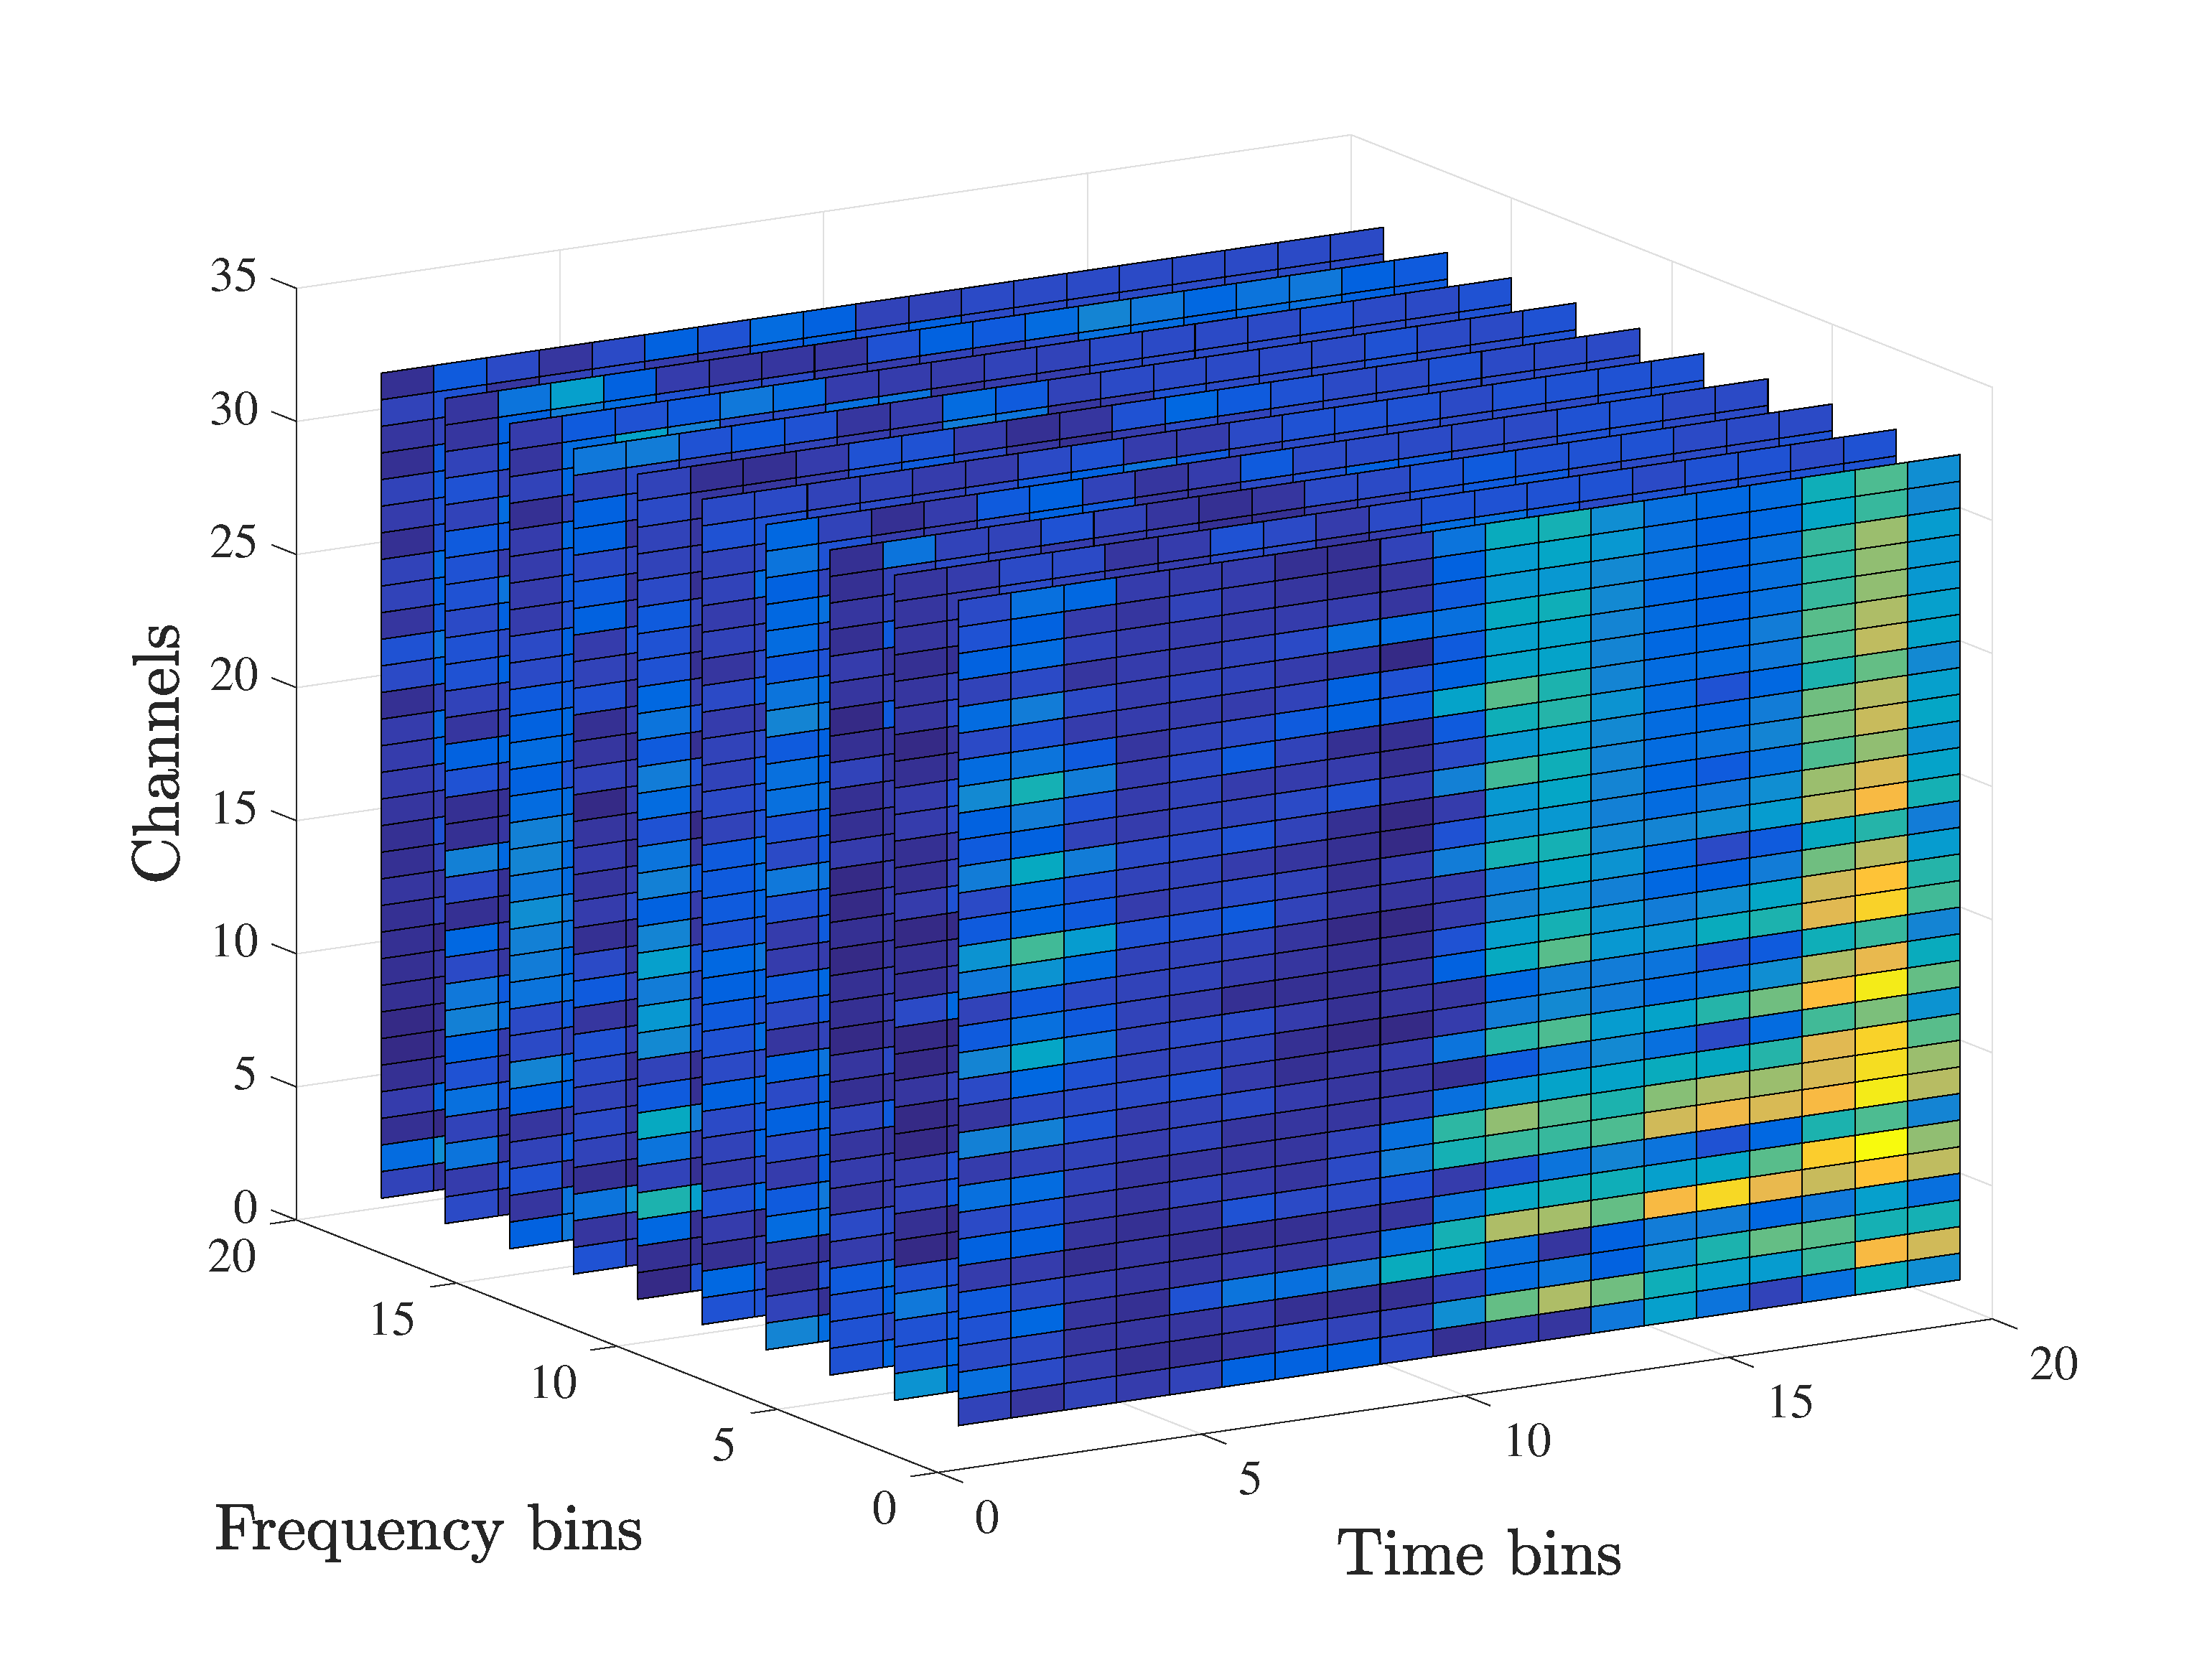
\includegraphics[width=\textwidth]{scalo_52_0_10_0.eps}
%     \vspace{-0.3cm}

    
% \column{0.55\textwidth}
% 	\includegraphics[width=0.85\textwidth]{taskla.png}
% \vspace{-0.3cm}
% \end{columns}
% \center{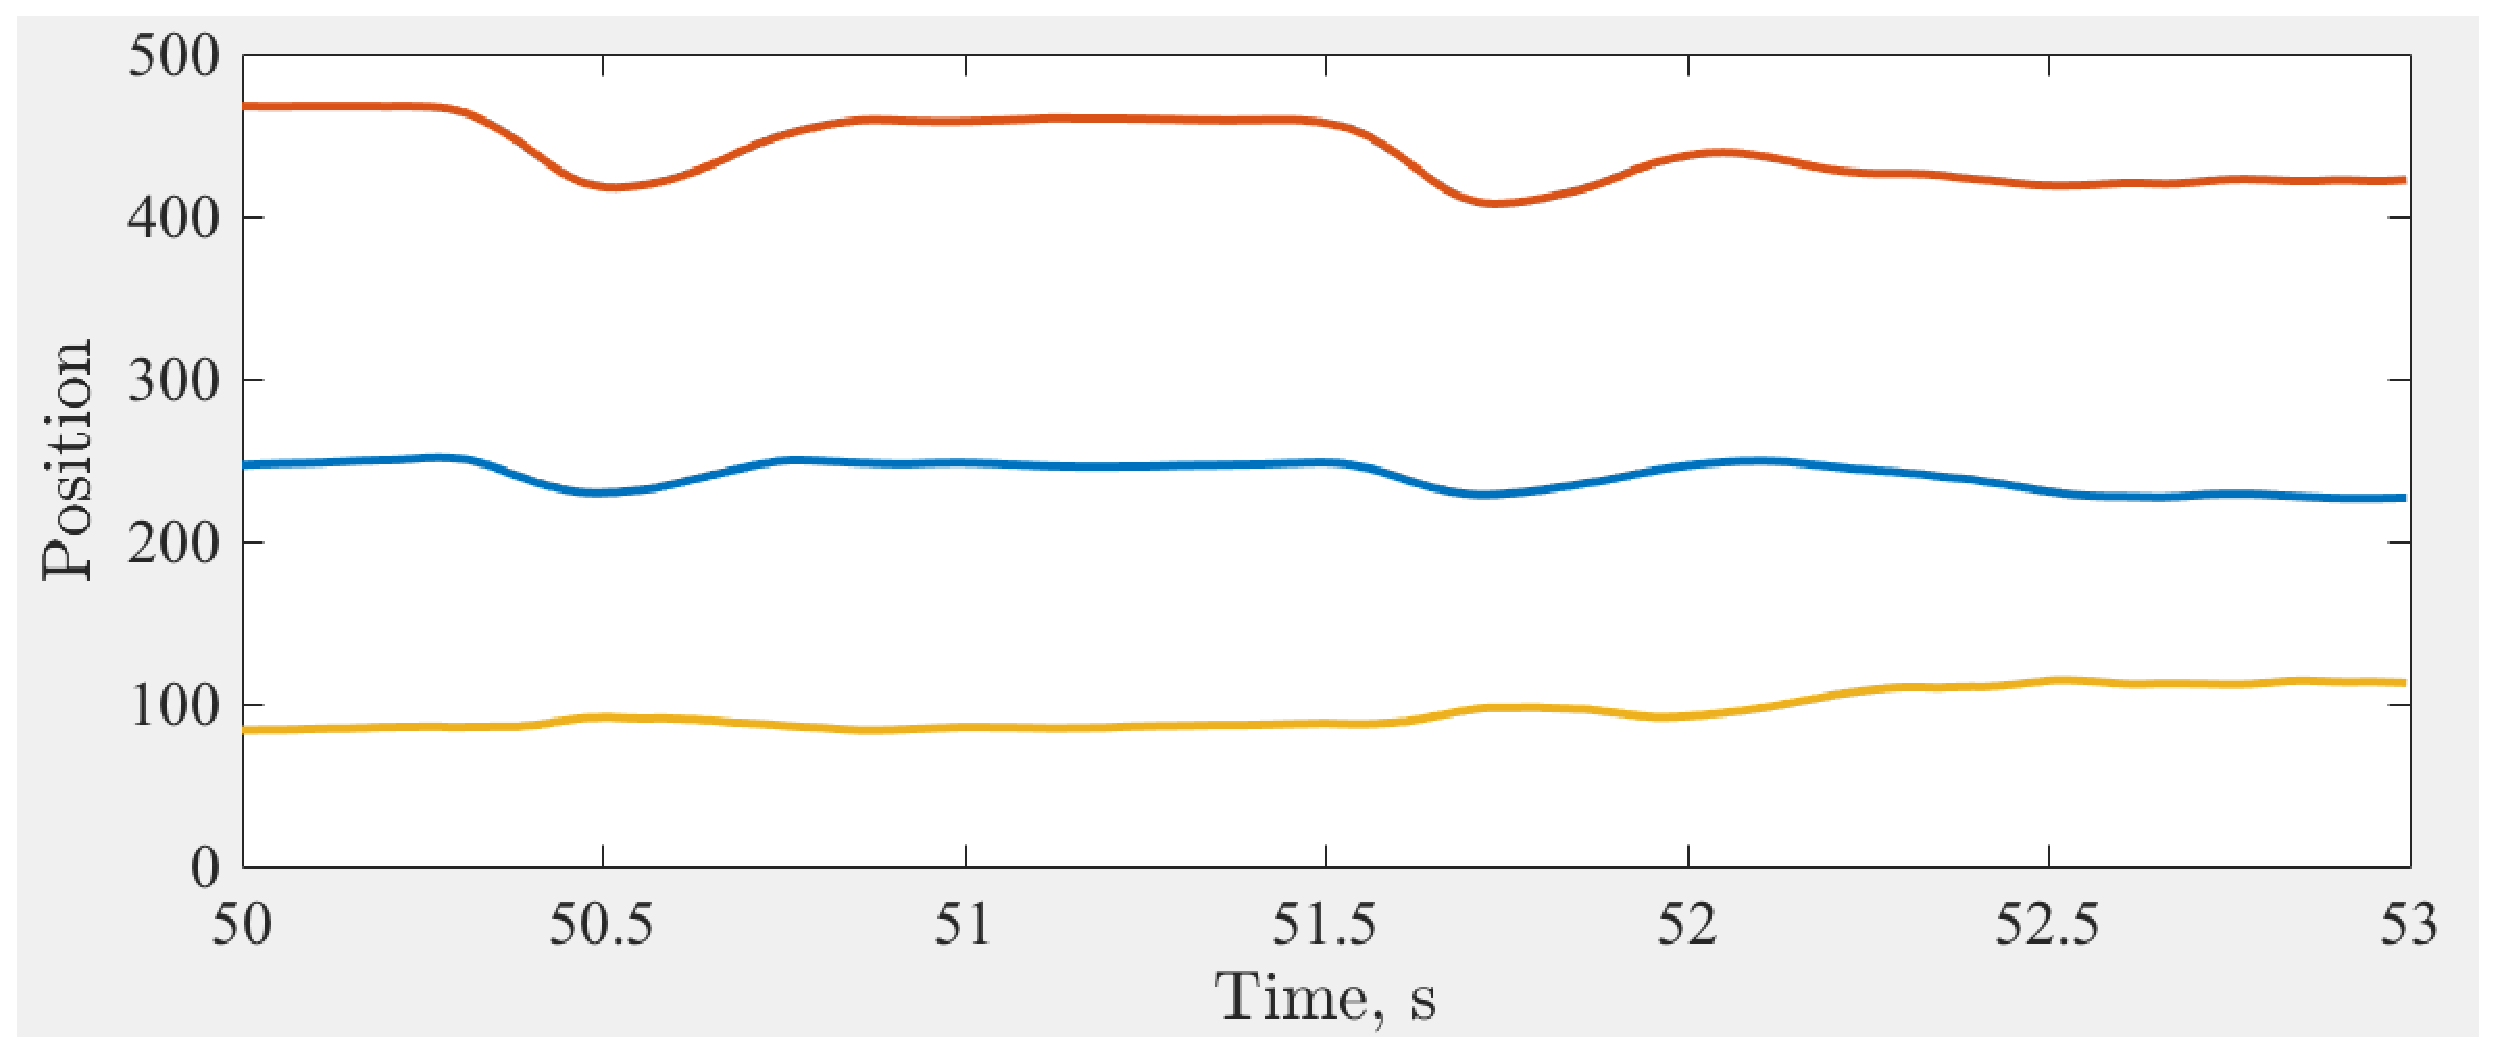
\includegraphics[width=0.8\textwidth]{LELB_50to53sPNG.eps}}

% }

% \end{frame}
%----------------------------------------------------------------------------------------------------------
\begin{frame}{Литература}
\begin{itemize}
  \item \footnotesize{Höskuldsson A. PLS regression methods //Journal of chemometrics. – 1988. – Т. 2. – №. 3. – С. 211-228.}
  \newline
  \item \footnotesize{Frank I. E. A nonlinear PLS model //Chemometrics and intelligent laboratory systems. – 1990. – Т. 8. – №. 2. – С. 109-119.}
  \newline
  \item \footnotesize{Rosipal R. Nonlinear partial least squares: An overview //Chemoinformatics and advanced machine learning perspectives. – 2010. – С. 169-189.}
  \newline
  % \item \footnotesize{Motrenko A., Strijov V. Multi-way Feature Selection for ECoG-based Hand Movement Prediction // Artificial Intelligence. - 2017. (Подготовлено)}
\end{itemize}
\end{frame}
%----------------------------------------------------------------------------------------------------------
\begin{frame}{Постановка задачи}

\textbf{Дано:}

Временной ряд 
$\mathbf{x} = [x_t]$,  $t = 1, \dots , n$, $x_t \in \mathbb{R}$. 

Требуется спрогнозировать следующие $r$ значений сигнала: 
$\mathbf{y} = [y_t]$,  $t = 1, \dots , r$, $y_t \in \mathbb{R}$. 

\begin{figure}[H]
  \centering
  \def\svgwidth{100mm}
  \includesvg{draw_object}
\end{figure}

Матрица плана:
$\mathbf{X} =  [\boldsymbol{\chi}_1, \dots,  \boldsymbol{\chi}_n]$


Матрица ответов:
$ \mathbf{Y}\in \mathbb{R}^n $

Выборка: 
$\mathfrak{D}=   \left( \mathbf{X}, \mathbf{Y}\right)$

\vspace{-0.5cm}
\begin{equation*}
	\left[ \mathbf{X \, | \, Y} \right] = 
	\begin{bmatrix}
        x_1 & \dots  & x_{n} & \vrule & y_1 & \dots  & y_{r}\\
        x_2 & \dots & x_{n + 1} & \vrule & y_2 & \dots  & y_{r+1}\\
        \vdots & \ddots & \vdots & \vrule & \vdots & \ddots & \vdots \\
        x_{m} & \dots  & x_{m+n-1} & \vrule & y_{m} & \dots  & y_{r+m-1}
    \end{bmatrix} = 
    \begin{bmatrix}
        \mathbf{x}_1 & \vrule & \mathbf{y}_{1}\\
        \mathbf{x}_{2} &\vrule & \mathbf{y}_{2}\\
        \vdots & \vrule &  \vdots \\
        \mathbf{x}_{m} & \vrule & \mathbf{y}_{m}
    \end{bmatrix}.
\end{equation*}


% $$ \boldsymbol{Theta}^* = \argmin_{\boldsymbol{Theta}}{ S(\mathbf{w}, A \, | \, \mathbf{X}, \mathbf{y}, \mathbf{f})}$$

% $S(\mathbf{w}, \mathcal{A} \, | \, \mathbf{X}, \mathbf{Y}, \mathbf{f}) = {\bigl\| \mathbf{Xw} - \mathbf{Y} \bigr\|}^2$, $\mathbf{f} (\mathbf{X}, \cal{A}, \mathbf{w}) = \mathbf{X}_{\mathcal{A}} \mathbf{w}$

% $$\mathcal{A}^* = \argmin_{\mathcal{A} \subseteq \mathcal{J}} \mathcal{Q} (\mathcal{A} \, | \, \mathbf{X}, \mathbf{Y})$$
\end{frame}
%----------------------------------------------------------------------------------------------------------
\begin{frame}{Авторегрессионная модель}
\vspace{-0.5cm}
\begin{equation*}
	\bY = \mathbf{f} (\bX,  \boldsymbol{\Theta}) + \varepsilon ( \mathbf{X} ),
\end{equation*} 

где  $\mathbf{f} (\bX,  \boldsymbol{\Theta}) = \mathbf{X} \boldsymbol{\Theta}$ -- модель.
% , $\boldsymbol{\Theta} \in \mathbb{R}^{n \times r}$ -- матрица параметров, $\epsilon(\mathbf{X})$ -- вектор регрессионных остатков.
\begin{figure}[H]
  \centering
  \def\svgwidth{100mm}
  \includesvg{forecasting_model}
\end{figure}
\begin{equation*}
	S(\boldsymbol{\Theta} | \mathfrak{D}) = {\bigl\| \mathbf{f}(\mathbf{X},  \boldsymbol{\Theta}) - \bY \bigr\| }_2^2 =  {\bigl\| \bX \boldsymbol{\Theta} - \bY \bigr\| }_2^2.
\end{equation*}
\begin{equation*}
	\boldsymbol{\Theta}^* = \argmin_{\boldsymbol{\Theta} \in \mathbb{R}^{n \times r}} S(\boldsymbol{\Theta} | \mathfrak{D}).
\end{equation*}

\end{frame}
%----------------------------------------------------------------------------------------------------------
% \begin{frame}{Мультиколлинеарные признаки}
% $\mathbf{X}= {[\boldsymbol{\chi}_1, \dots , \boldsymbol{\chi}_{n}]}$~--- матрица плана.

% $\mathcal{J} = \{1, \dots , n \}$~--- множество индексов признаков. 

% \begin{block}{Мультиколлинеарные признаки} 
% 	Признаки из индексного подмножества $\mathcal{A} \subseteq \mathcal{J}$ называются \textit{мультиколлинеарными}, если существуют $j \in \mathcal{A}$, $\lambda_k \in \mathbb{R}$ и достаточно малое $\delta > 0$:
% 	\begin{equation*}
% 		{\left\| \boldsymbol{\chi}_j - \sum_{k\in \mathcal{A} \setminus j} \lambda_k \boldsymbol{\chi}_k \right\| }_2^2 < \delta.
% 	\end{equation*}
% \end{block}
% \vspace{-0.7cm}
% % \begin{block}{Активные признаки}
% % 	Признаки, которым соответствуют ненулевые строки матрицы $\boldsymbol{\Theta}$, называются \emph{активными}. Множество всех индексов активных признаков $\mathcal{A}$.
% % \end{block}
% % \vspace{-0.2cm}
% \begin{block}{Задача отбора признаков}
% 	% \vspace{-0.5cm}
% 	\begin{equation*}
% 		{\mathcal{A}}^{*} = \argmin_{\mathcal{A} \in \mathcal{J}} \mathcal{Q} (\mathcal{A} \, | \, \mathfrak{D}_{\mathcal{C}}), 
% 	\end{equation*}
% 	где $\mathcal{Q}: \, \mathcal{A} \rightarrow \mathbb{R}$ -- критерий качества. 
% \end{block}

% \end{frame}
%----------------------------------------------------------------------------------------------------------
% \begin{frame}{Критерии}
% % $\mathbf{X}_\mathcal{A}$ -- матрица отобранных признаков.\\
% % $\mathbf{Y}_\mathcal{A}$ -- проекция значений матрицы $\mathbf{Y}$ из контрольной выборки на пространство меньшей размерности.\\
% % $r = S\left(\boldsymbol{\Theta}^{*}|(\mathbf{X}, \mathbf{Y})\right)$, $r_{\mathcal{A}} = S \left(  \boldsymbol{\Theta}^{*}|(\mathbf{X}_{\mathcal{A}}, \mathbf{Y}_{\mathcal{A}}) \right)$.


% \begin{enumerate}
% \item Критерий Маллоуза $C_p$. 
% % позволяет достичь компромисса между величиной $\rss$ и количеством используемых переменных $p$, а также ликвидировать возможную коллинеарность признаков. Величина $C_p$ определяется следующим образом:
% \[
% C_p = \frac{RSS_p}{RSS} - m + 2p,
% \]
% где $RSS_p$~--- это величина, аналогичная $RSS$, найденная при использовании $p$ признаков. 
% % Меньшие значения $C_p$ соответствуют лучшему набору признаков. 
% \item Критерии сравнения методов выбора признаков $d = p - h$,
% 	\begin{equation*}
% 		h = \argmax\limits_{S(\mathcal{J}_h, \boldsymbol{\Theta}_h, \mathfrak{D}) \le s_0} |\mathcal{J}_h|,
% 	\end{equation*}
% 	где $S(\mathcal{J}_h, \boldsymbol{\Theta}_h, \mathfrak{D})$~--- функция ошибки, $s_0$~--- некоторое предельное значение.

% 	\footnotesize{A. M. Katrutsa, V. V. Strijov. Stresstest procedure for feature selection algorithms // Chemometrics and Intelligent Laboratory Systems}  

% \end{enumerate} 

% \end{frame}
%----------------------------------------------------------------------------------------------------------
\begin{frame}{Метод PLSR}
\vspace{0.5cm}
\begin{columns}
\column{0.52\textwidth}
\begin{tikzpicture}
  % \node (x) {$\bX$};
  \node (tp) {$\bX = \bT \bP^{T} + \bE$};
  \node (xp) [below of=tp] {$\bX \bP \not= \bT$};
  % \node (y) [right of=x, xshift=4cm] {$\bY$};
  \node (uq) [right of=tp, xshift=3cm] {$\bY = \bU \bQ^{T} + \bF$};
  \node (yq) [below of=uq] {$\bY \bQ \not= \bU$};
  \node (td) [below of=xp, xshift=2cm, yshift=-0.5cm] {$\bU = \bT \bD + \bZ$};

  % \draw [arrow] (xp) -- (td);
  \path [draw, ->] +(-0.5,-1.2) -- node [above] {$\bw$}
      +(1.8,-2.3);
  \path [draw, ->] +(3.4,-1.2) -- node [above] {$\bc$}
      +(1.2,-2.3);
\end{tikzpicture}

\column{0.48\textwidth}
\centerline{$\bX \in \mathbb{R}^{n \times m}$, $\bT \in \mathbb{R}^{n \times p}$}
\centerline{$ \bY \in \mathbb{R}^{n \times r}, \bU \in \mathbb{R}^{n \times r}$}

% \begin{equation*}
% 	\bX = \mathbf{T P^{\T} + E},
% 	\quad \quad
% 	\bY = \mathbf{U Q^{\T} + F}
% \end{equation*}
\end{columns}
% \centerline{$\bX \in \mathbb{R}^{n \times m}$, $\bT \in \mathbb{R}^{n \times p}, \quad \quad \bY \in \mathbb{R}^{n \times r}, \bU \in \mathbb{R}^{n \times r}$}
\vspace{0.5cm}
Используется итеративный алгоритм,  инициализиируем $\bu:=\by_1$
% , который находит векторы весов $\bw, \bc$

	\begin{multicols}{2}
	\begin{enumerate}
		\item $\bw = \bX^{\T} \bu / \|\bX^{\T} \bu\|$
    \vspace{-0.2cm}
		\item $\bt = \bX \bw$
		\item $\bc = \bY^{\T} \bt / \|\bY^{\T} \bt\|$
    \vspace{-0.2cm}
		\item $\bu = \bY \bc$
	\end{enumerate}
	\end{multicols}
\vspace{-0.7cm}
\begin{equation*}
  \bp = \bX^{\bT} \bt/\| \bX^{\bT} \bt\|, \quad \bq = \bY^{\T} \bu / \| \bY^{\T} \bu\|
\end{equation*}

Полученное значение $\bp$ максимизирует ковариацию между новыми признаками и ответом
  \[
    [Cov( \bt, \bu)]^2 = [Cov(\bX \bw, \bY \bc)]^2 
    % = \max\limits_{ |\mathbf{r}| = |\bs| = 1}[Cov(\bX \mathbf{r}, \bY \bs)]^2
  \]

\end{frame}
%----------------------------------------------------------------------------------------------------------
% \begin{frame}{Мультиколлинеарность в $\bX$ и $\bY$}

% \tikzstyle{sensor_x}=[draw, fill=blue!0, text width=6.5em, 
%     text centered, minimum height=8em,drop shadow]
% \tikzstyle{sensor_y}=[draw, fill=blue!0, text width=5em, 
%     text centered, minimum height=8em,drop shadow]

% \footnotesize{
% \def\blockdist{2.3}
% \def\edgedist{2.5}

% \hspace{1cm}
% \begin{tikzpicture}
%     \node (x) [sensor_x]  {$\bX$};
%     \path (x.south)+(0,-3) node (tilde_x) [sensor_x] {$\tilde \bX$};
%     \path (x.east)+(5,0) node (y) [sensor_y] {$\bY$};
%     \path (y.south)+(0,-3) node (tilde_y) [sensor_y] {$\tilde \bY$};
%     \path (tilde_x.south)+(0,-0.7) node (x_form) {$\tilde \bX = \bT \bP^{T} + \bE$};
%     \path (tilde_y.south)+(0,-0.7) node (y_form) {$\tilde \bY = \bU \bQ^{\T} + \bM$};
%     \path (tilde_x.south)+(3.4,-1) node (u_form) {$\bU = \bT \bD + \bZ$};


%     \path [draw, ->] (x.south) -- node [right] {$f_x(\bX, \bv_x)$} 
%         (tilde_x.north);
%     \path [draw, ->] (y.south) -- node [right] {$f_y(\bY, \bv_y)$} 
%         (tilde_y.north);
%     %tilde X
%     \path [draw, -] +(1.25,-3) -- node [right] {$\bt$}
%     	+(1.25,-5.6);
%     \path [draw, -] +(1.2,-5.7) -- node [below] {$\bp$}
%     	+(-1.2,-5.7); 
%    	%tilde Y
%     \path [draw, -] +(5.17,-3) -- node [left] {$\bu$}
%     	+(5.17,-5.6);
%     \path [draw, -] +(5.3,-5.7) -- node [below] {$\bq$}
%     	+(7.1,-5.7);

%     \path [draw, ->] +(1.15,-5.6) -- node [above] {$\bw$}
%     	+(3.23,-6.45);
%     \path [draw, ->] +(5.25,-5.6) -- node [above] {$\bc$}
%     	+(2.7,-6.45);
% \end{tikzpicture}
% }
% \end{frame}
%----------------------------------------------------------------------------------------------------------
\begin{frame}{Мультиколлинеарность в $\bX$ и $\bY$}


\tikzstyle{sensor_x}=[draw, fill=blue!0, text width=4em, 
    text centered, minimum height=5em,drop shadow]
\tikzstyle{sensor_y}=[draw, fill=blue!0, text width=2.7em, 
    text centered, minimum height=5em,drop shadow]

\footnotesize{
\def\blockdist{2.3}
\def\edgedist{2.5}

\hspace{1cm}
\begin{tikzpicture}
    \node (x) [sensor_x]  {$\bX$};
    \path (x.south)+(0,-2) node (tilde_x) [sensor_x] {$\tilde \bX$};
    \path (x.east)+(4,0) node (y) [sensor_y] {$\bY$};
    \path (y.south)+(0,-2) node (tilde_y) [sensor_y] {$\tilde \bY$};
    \path (tilde_x.south)+(0,-0.8) node (x_form) {$\tilde \bX = \bT \bP^{T} + \bE$};
    \path (tilde_y.south)+(0.4,-0.8) node (y_form) {$\tilde \bY = \bU \bQ^{\T} + \bM$};
    \path (tilde_x.south)+(2.5,-1.3) node (u_form) {$\bU = \bT \bD + \bZ$};


    \path [draw, ->] (x.south) -- node [right] {$f_x(\bX, \bv_x)$} 
        (tilde_x.north);
    \path [draw, ->] (y.south) -- node [right] {$f_y(\bY, \bv_y)$} 
        (tilde_y.north);
    %tilde X
    \path [draw, -] +(0.95,-2) -- node [right] {$\bt$}
      +(0.95,-3.6);
    \path [draw, -] +(0.8,-3.8) -- node [below] {$\bp$}
      +(-0.8,-3.8); 
    %tilde Y
    \path [draw, -] +(4.05,-2) -- node [left] {$\bu$}
      +(4.05,-3.6);
    \path [draw, -] +(4.2,-3.8) -- node [below] {$\bq$}
      +(5.4,-3.8);

    \path [draw, ->] +(0.8,-3.6) -- node [above] {$\bw$}
      +(2.31,-4.8);
    \path [draw, ->] +(4.17,-3.6) -- node [above] {$\bc$}
      +(1.9,-4.8);
\end{tikzpicture}
}
\end{frame}
%----------------------------------------------------------------------------------------------------------
% \begin{frame}{Преобразование $\bY$}


% \begin{tikzpicture}
% 	% \node (x) {$\bX$};
% 	\node (tp) {$\tilde \bX$};
%   \node (xp) [below of=tp] {$\tilde \bX = \bT \bP^{T} + \bE$};
% 	% \node (y) [right of=x, xshift=4cm] {$\bY$};
%   \node (uq) [right of=tp, xshift=3cm] {$\tilde \bY$};
%   \node (yq) [below of=uq] {$\tilde \bY = \bU \bQ^{T} + \bF$};
%   \node (td) [below of=xp, xshift=2cm, yshift=-0.5cm] {$\bU = \bT \bD + \bZ$};

%   % \draw [arrow] (xp) -- (td);
%   \path [draw, ->] +(-0.5,-1.2) -- node [above] {$\bw$}
%       +(1.8,-2.3);
%   \path [draw, ->] +(3.4,-1.2) -- node [above] {$\bc$}
%       +(1.2,-2.3);
% \end{tikzpicture}

% \end{frame}
%----------------------------------------------------------------------------------------------------------
\begin{frame}{Преобразование $\bY$}

\begin{itemize}
\item Криволинейное преобразование целевой переменной с вектором параметров $\bv$
	\begin{equation*}
	\label{transf_y}
		\breve \bY = g (\bY, \bv).
	\end{equation*}

Настройка параметров $\bv$ с помощью градиентного спуска. 


\item Нелинейное преобразование целевой переменной с помощью непараметрической функции
	\begin{equation*}
		\tilde \bY = h (\breve \bY) = h( g( \bY)) = f(\bY)
	\end{equation*}

\end{itemize}


\begin{block}{Схема композиции преобразований}
	\[\begin{diagram}
	\node{\bY}
	\arrow{e,t}{g(\bY, \bv)}
	\node{\breve \bY}
	\arrow{e,t}{h(\breve \bY)}
	\node{\tilde \bY}
	\end{diagram}
  \quad \Rightarrow \quad
  \begin{diagram}
  \node{\bY}
  \arrow{e,t}{f(\bY, \bv)}
  \node{\tilde \bY}
  \end{diagram}\]
\end{block}

\end{frame}
%----------------------------------------------------------------------------------------------------------
\begin{frame}{Преобразование $\bX$}
\begin{itemize}
\item Криволинейное преобразование зависимой переменной с вектором параметров $\bv$
	\begin{equation*}
	\label{inner_pls_nl}
		\breve \bX = g(\bX, \bv).
	\end{equation*}

% Модификация в алгоритме PLS:
% 	\begin{equation*}
% 		\bu = \bX \bw  + \bz \quad \to \quad \bu = g(\bX, \bv)\bw  + \bz.
% 	\end{equation*} 

\item Нелинейное преобразование зависимой переменной с помощью непараметрической функции
	\begin{equation*}
	\label{inner_pls_nl}
		\tilde \bX = h(\breve \bX) = h( g(\bX)) = f(\bX).
	\end{equation*}
	

\begin{block}{Схема композиции преобразований}
  \[\begin{diagram}
  \node{\bX}
  \arrow{e,t}{g(\bX, \bv)}
  \node{\breve \bX}
  \arrow{e,t}{h(\breve \bX)}
  \node{\tilde \bX}
  \end{diagram}
  \quad \Rightarrow \quad
  \begin{diagram}
  \node{\bX}
  \arrow{e,t}{f(\bX, \bv)}
  \node{\tilde \bX}
  \end{diagram}\]
\end{block}
% Модификация в алгоритме PLS:
% 	\begin{equation*}
% 		\bu = \bX \bw  + \bz \quad \to \quad \bu = h(\bX)\bw  + \bz.
% 	\end{equation*}
\end{itemize}

\end{frame}
%----------------------------------------------------------------------------------------------------------
\begin{frame}{Примеры преобразований}

\begin{table}[h]
\centering
\label{table_functions}
\begin{tabular}{|l|l|l|}
\hline
\textbf{№} & \textbf{Функция}                                  & \textbf{Параметры} \\ \hline
1          & $g(x) = \text{sign}(x)\exp(a)(\exp(b|x|) - 1)$          & $a, b > 0$         \\ \hline
2          & $g(x) = \text{sign}(x)\exp(a)(\exp(b\ln(1+ \,|x|) - 1)$ & $a, b > 0$         \\ \hline
3          & $g(x) = \text{sign}(x)\exp(a)(\exp(b|x|^{1/2}) - 1)$    & $a, b > 0$         \\ \hline
4          & $g(x) = \text{sign}(X)\exp(a)(\exp(b|x|^{1/3}) - 1)$    & $a, b > 0$         \\ \hline
5          & $g(x) = \text{sign}(x)\exp(a)(\exp(b|x|^{1/4}) - 1)$    & $a, b > 0$         \\ \hline
6          & $g(x) = \text{sign}(x)\exp(a)(\exp(b|x|^{2}) - 1)$      & $a, b > 0$         \\ \hline
\end{tabular}
\caption{Криволинейные преобразования}
\end{table}


\end{frame}
%----------------------------------------------------------------------------------------------------------
\begin{frame}{Алгоритм cnlPLS для зависимой переменной}

Криволинейное + нелинейное преобразование~$f$ в пространстве целевой  переменной $\bY$ в алгоритме PLSR
\newline
\newline
Инициализировать $\bv$, $\bY:=\by_1$, $\bu_0 := f(\bY, \bv)$,  выполнить в цикле
	\begin{multicols}{2}
	\begin{enumerate}
		\item $\bw = \bX^{\T} \bu_0 / \|\bX^{\T} \bu_0 \|$

		\item $\bt = \bX \bw$

    \item $\tilde \bY = f(\bY, \bv)$

		\item $\bc = \tilde \bY^{\T} \bt / \| \tilde \bY^{\T} \bt\| $

		\item $\bu = \tilde \bY \bc$

		\item $\be = \bu - \bu_{0}$ 

		\item $\bJ = \partial \bu / \partial \bv$

		\item $\Delta \bv = (\bJ^{\T} \bJ)^{-1} \bJ^{\T} \be$

		\item $\bv = \bv + \Delta \bv$, $\| \bv \| \to 1$

    \item $\bu_0 := \bu$

	\end{enumerate}
	\end{multicols}
  Вычислить $\bp = \bX^{\bT} \bt/\| \bX^{\bT} \bt\|, \ \bq = \tilde \bY^{\T} \bu / \| \tilde \bY^{\T} \bu\|$.
\end{frame}
%-----------------------------------------------------------------------------------------------------
\begin{frame}{Эксперимент}

\begin{itemize}
\item данные содержат временные ряды электроэнергии, погоду (температура, осадки, сила ветра, влажность, солнечная энергия), график отпусков;
\item потребление энергии измерялось ежечасно с 1999 по 2004 год, 52512 наблюдений;
\item погода измерялась ежедневно, 2188 наблюдений.
\end{itemize}
\vspace{-0.3cm}
  \begin{figure}
    \includegraphics[width=1\linewidth]{\hdir/electricity.png}
  % \caption{}
  \end{figure}
  \vspace{-0.5cm}
  \center{Рисунок: Временной ряд потребления электроэнергии}
\end{frame}
%-----------------------------------------------------------------------------------------------------
% \begin{frame}{Эксперимент}

% \includegraphics[width=0.9\textwidth]{primates_pic.png}

% \begin{itemize}    
% %\item Epidural (64 electrodes): 2 monkeys, 10 records for each monkey, taken within 3 month (some on the same day).

% \item Субдуральные (32 электрода): 2 обезьяны, 3 и 5 записей, снятые в течение 7 месяцев.
% \item Каждая запись измеряет около 1000 секунд ЭКГ и данные движения (запястья, локти и плечи), отснятые на частотах 1 кГц и 120 Гц соответственно.

% \end{itemize}

% \begin{block}{Ошибки}
% \begin{equation*}
% 	RSS = \sum\limits_{i = 1}^r \varepsilon^2(\bx_i), \quad MAPE = \frac1{r}\sum\limits_{i = 1}^r \frac{|\varepsilon(\bx_i)|}{|\by_i|}
% 	% , \quad sMAPE = \frac1{r}\sum\limits_{i = 1}^r \frac{2|\varepsilon(\bx_i)|}{|\hat{\by}_i + \by_i|}
% \end{equation*}
% \end{block}

% \end{frame}
%----------------------------------------------------------------------------------------------------------
% \begin{frame}{Кросс-корреляция между каналами}

% \Wider[2em]{ \footnotesize

% \begin{columns}[c]
% \column{0.05\textwidth}
% \column{0.45\textwidth}
% \includegraphics[width=0.8\textwidth]{electrodes.png}

% \column{0.5\textwidth}
% \includegraphics[width=0.8\textwidth]{el_corr_td0_cb.png} \\ 
% % \vspace{-0.5cm}
% \includegraphics[width=0.8\textwidth]{el_corr_td100_cb.png}
% \end{columns}

% }

% % Коэффициент корреляции 
% % \begin{equation*}
% %   \text{corr} (\hat{\bY}, \bY) = \frac{\text{cov}(\hat{\by},\by)}{\sqrt{\text{cov}(\hat{\by},\by)\text{cov}(\by,\by)}}
% % \end{equation*}

% \end{frame}
%----------------------------------------------------------------------------------------------------------
\begin{frame}{Предсказания на разные временные отрезки}
   
  \hspace*{-1.1cm}
  \vspace*{0cm}
    \centering
      \includegraphics[width=0.4\textwidth]{\hdir/oneday.png}
      \hspace*{-0.2cm}
      \includegraphics[width=0.4\textwidth]{\hdir/twodays.png}
      \hspace*{-0.2cm}
      \includegraphics[width=0.4\textwidth]{\hdir/fivedays.png}

    \hspace*{-1.1cm}
    \vspace{1cm}
      \centering
      \includegraphics[width=0.4\textwidth]{\hdir/tendays.png}
      \hspace*{-0.2cm}
      \includegraphics[width=0.405\textwidth]{\hdir/twentydays.png}
      \hspace*{-0.2cm}
      \includegraphics[width=0.42\textwidth]{\hdir/month.png}


\end{frame}%-----------------------------------------------------------------------------------------------------
\begin{frame}{Зависимость ошибки от числа компонент для разных функций преобразования}
\hspace*{-1.1cm}
  \vspace*{0cm}
    \centering
      \includegraphics[width=0.4\textwidth]{\hdir/exp_abs_x.png}
      \hspace*{-0.2cm}
      \includegraphics[width=0.4\textwidth]{\hdir/exp_log_x.png}
      \hspace*{-0.2cm}
      \includegraphics[width=0.4\textwidth]{\hdir/exp_x_1_2.png}

    \hspace*{-1.1cm}
    \vspace{1cm}
      \centering
      \includegraphics[width=0.4\textwidth]{\hdir/exp_x_1_3.png}
      \hspace*{-0.2cm}
      \includegraphics[width=0.4\textwidth]{\hdir/exp_x_1_4.png}
      \hspace*{-0.2cm}
      \includegraphics[width=0.4\textwidth]{\hdir/exp_x_2.png}
\end{frame}
%-----------------------------------------------------------------------------------------------------
\begin{frame}{Результаты}


\footnotesize{
\begin{table}
\hspace*{-0.5cm}
\begin{tabular}{|l|l|l|l|l|}
\hline
\textbf{Алгоритм}                                                                                  & \textbf{N=3}     & \textbf{N=5}     & \textbf{N=10}    & \textbf{N=20}    \\ \hline
PLS                                                                                                & 0,00404          & 0,00337          & \textbf{0,00151} & 0,00135          \\ \hline
\begin{tabular}[c]{@{}l@{}}cnlPLS\\ $g(x) = \text{sign}(x)e^a(\exp(b|x|) - 1)$\end{tabular}          & 0.00529          & 0.00514          & 0.00536          & 0.00506          \\ \hline
\begin{tabular}[c]{@{}l@{}}cnlPLS\\ $g(x) = \text{sign}(x)e^a(\exp(b\ln(1+ \,|x|) - 1)$\end{tabular} & 0.00362          & 0.00386          & 0.00326          & 0.00317          \\ \hline
\begin{tabular}[c]{@{}l@{}}cnlPLS\\ $g(x) = \text{sign}(x)e^a(\exp(b|x|^{1/2}) - 1)$\end{tabular}    & 0.00272          & 0.00236          & 0.00287          & \textbf{0.00128} \\ \hline
\begin{tabular}[c]{@{}l@{}}cnlPLS\\ $g(x) = \text{sign}(x)e^a(\exp(b|x|^{1/3}) - 1)$\end{tabular}    & \textbf{0.00241} & \textbf{0.00233} & 0.00221          & 0.00173          \\ \hline
\begin{tabular}[c]{@{}l@{}}cnlPLS\\ $g(x) = \text{sign}(x)e^a(\exp(b|x|^{1/4}) - 1)$\end{tabular}    & 0.00796          & 0.00768          & 0.00737          & 0.00803          \\ \hline
\begin{tabular}[c]{@{}l@{}}cnlPLS\\ $g(x) = \text{sign}(x)e^a(\exp(b|x|^{2}) - 1)$\end{tabular}      & 0.00816          & 0.00798          & 0.00796          & 0.00775          \\ \hline
\end{tabular}
\caption{Значения ошибки MSE для разных чисел компонент и разных функций}
\end{table}
}
\end{frame}
%----------------------------------------------------------------------------------------------------------
% \begin{figure}
%     \centering
%     \begin{subfigure}[b]{0.4\textwidth}
%         \includegraphics[width=\textwidth]{exp_abs_x.png}
%         \caption{$g(x) = \sign(x) e^a(\exp(b|x|) - 1)$}
%         \label{fig:exp_abs_x}
%     \end{subfigure}
%     ~ %add desired spacing between images, e. g. ~, \quad, \qquad, \hfill etc. 
%       %(or a blank line to force the subfigure onto a new line)
%     \begin{subfigure}[b]{0.4\textwidth}
%         \includegraphics[width=\textwidth]{exp_log_x.png}
%         \caption{$g(x) = \sign(x)e^a(\exp(b\ln(1+ \,|x|) - 1)$}
%         \label{fig:exp_log_x}
%     \end{subfigure}
%     ~ %add desired spacing between images, e. g. ~, \quad, \qquad, \hfill etc. 
%     %(or a blank line to force the subfigure onto a new line)
%     \begin{subfigure}[b]{0.4\textwidth}
%         \includegraphics[width=\textwidth]{exp_x_1_2.png}
%         \caption{$g(x) = \sign(x)e^a(\exp(b|x|^{1/2}) - 1)$}
%         \label{fig:exp_x_1_2}
%     \end{subfigure}
%     \begin{subfigure}[b]{0.4\textwidth}
%         \includegraphics[width=\textwidth]{exp_x_1_3.png}
%         \caption{$g(x) = \sign(x)e^a(\exp(b|x|^{1/3}) - 1)$ }
%         \label{fig:exp_x_1_3}
%     \end{subfigure}
%     ~ %add desired spacing between images, e. g. ~, \quad, \qquad, \hfill etc. 
%       %(or a blank line to force the subfigure onto a new line)
%     \begin{subfigure}[b]{0.4\textwidth}
%         \includegraphics[width=\textwidth]{exp_x_1_4.png}
%         \caption{$g(x) = \sign(x)e^a(\exp(b|x|^{1/4}) - 1)$}
%         \label{fig:exp_x_1_4}
%     \end{subfigure}
%     ~ %add desired spacing between images, e. g. ~, \quad, \qquad, \hfill etc. 
%     %(or a blank line to force the subfigure onto a new line)
%     \begin{subfigure}[b]{0.4\textwidth}
%         \includegraphics[width=\textwidth]{exp_x_2.png}
%         \caption{$g(x) = \sign(x)e^a(\exp(b|x|^{2}) - 1)$}
%         \label{fig:exp_x_2}
%     \end{subfigure}
%     \caption{Зависимость ошибки от числа компонент в алгоритме cnlPLS для разных функций}\label{fig:animals}
% \end{figure}
% \end{frame}
%-----------------------------------------------------------------------------------------------------
% \begin{frame}{Примеры прознозирования}


% \includegraphics[width=\textwidth]{2D_0p65_Tucker_1_1_50feats_25sm.png}


% \end{frame}
%----------------------------------------------------------------------------------------------------------
\begin{frame}{Результаты, выносимые на защиту}
\begin{itemize}
  \item Предложены алгоритмы прогнозирования временных рядов.
  \smallskip
  \item Предложены методы снижения мультиколлинеарности в пространстрах зависимой и независимой переменной.
  \medskip
  \item Выполнена программная реализация и проведены численные эксперименты, показавшие повышение качества решения задачи прогнозирования сигналов.
\end{itemize}

\end{frame}
%----------------------------------------------------------------------------------------------------------
\end{document} 